% A simple graph with straight and bend arrows and loops
% Stefan Kottwitz
\documentclass{article}
\usepackage{tikz}
\usetikzlibrary{arrows}
\begin{document}
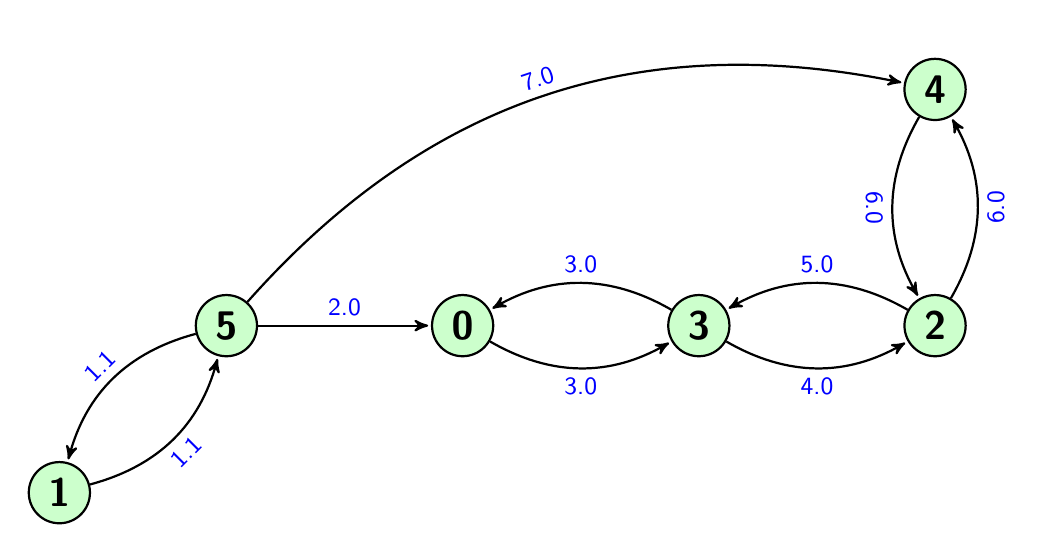
\begin{tikzpicture}[->,>=stealth',shorten >= 1pt,auto,node distance=3cm,
  thick,main node/.style={circle,fill=green!20,draw,font=\sffamily\Large\bfseries}]

  \node[main node] (1) {1};
  \node[main node] (5) [above right of=1] {5};
  \node[main node] (0) [	  right of=5] {0};
  \node[main node] (3) [      right of=0] {3};
  \node[main node] (2) [      right of=3] {2};
  \node[main node] (4) [above       of=2] {4};

  \path[every node/.style={font=\sffamily\small}]
  	(1) edge [bend right] node [blue, pos=0.5, sloped, below] {1.1} (5)
  	(5) edge [bend right] node [blue, pos=0.5, sloped, above] {1.1} (1)
  	(5) edge 			  node [blue, pos=0.5, sloped, above] {2.0} (0)
  	(0) edge [bend right] node [blue, pos=0.5, sloped, below] {3.0} (3)
  	(3) edge [bend right] node [blue, pos=0.5, sloped, above] {3.0} (0)
  	(3) edge [bend right] node [blue, pos=0.5, sloped, below] {4.0} (2)
  	(2) edge [bend right] node [blue, pos=0.5, sloped, above] {5.0} (3)
  	(2) edge [bend right] node [blue, pos=0.5, sloped, below] {6.0} (4)
  	(4) edge [bend right] node [blue, pos=0.5, sloped, below] {6.0} (2)
  	(5) edge [bend left] node [blue, pos=0.5, sloped, above] {7.0} (4);
    
\end{tikzpicture}
\end{document}